\documentclass{article}

% Packages
\usepackage{graphicx} % For including images
\usepackage{listings} % For including code snippets
\usepackage{xcolor}   % For custom colors

% Document Metadata
\title{Single-Cycle Datapath Simulator for LEGv8 Architecture}
\author{Graham Pellegrini}
\date{\today}

\begin{document}

\maketitle

\tableofcontents

\newpage

\section{Introduction}
The Single-Cycle Datapath Simulator for LEGv8 Architecture is a C++ program designed to simulate the behavior of a single-cycle processor implementing a subset of the LEGv8 instruction set architecture. The simulator is capable of loading a program from a file, executing the respective modules that make up the processor, and outputting the results of the simulation after each cycle. The simulator is designed to be modular, allowing for easy extension to support additional instructions and features.

\section{Implementation Details}

The implementation of the simulator is divided into several modules, each responsible for a specific aspect of the simulation:

\subsection{Main Class: MNE2701\_Legv8\_Sim}
This class is responsible for initializing the simulator and executing the sequential nature of the single-cycle processor.\\

Here all the processor modules are initialized, as well as data such as the register array, memory array, program counter, and instruction register.\\

\begin{figure}[htbp]
    \centering
    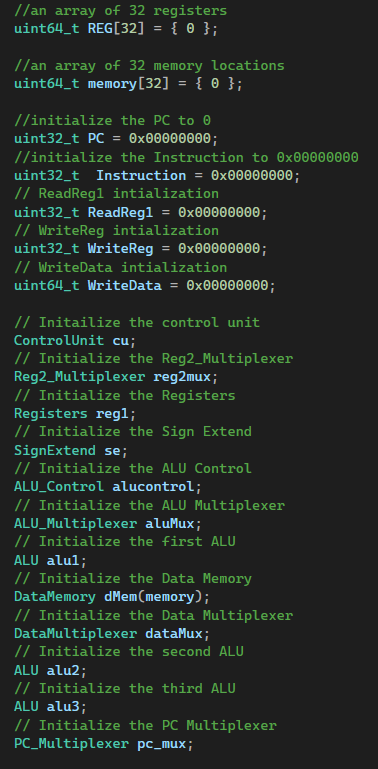
\includegraphics[width=0.6\textwidth]{screen_dumps/main_initializing.png}
    \caption{Main Class Initialization}
    \label{fig:1}
\end{figure}

The simulator then enters a loop where it fetches, decodes, and executes instructions until the program counter reaches the end same index as the Instruction count. Note that the program counter is incremented by 4 after each instruction is executed.\\

Inside the loop, the simulator links the modules together by passing the necessary data between them. Finally outputting the states of the registers and memory after every cycle.\\

\subsection{Instruction Fetch and Execute Module: Instruction\_Memory}
The Instruction Memory module is responsible for loading and storing instructions from the input .text file. It is initialized once as it attempts to load the instructions from the file into an array.\\

Then the moduled is called to use function readaddress() to fetch the instruction at the current program counter index.\\

A further function getInstructionCount() is used to return the number of instructions in the array. This is used to determine when the program counter has reached the end of the program.\\

\subsection{Control Unit Module: ControlUnit}
The Control Unit module generates control signals for the processor based on the opcode of the instruction. The control unit module is initialized once and then called to generate the control signals for each instruction.\\

Within the setControlSignals() function, two operations are performed. The first we distinguish between the different types of instructions using an if else statement. Extracting the 11 bits of the opcode of the instruction with the appropriate bit field to be able determine the type of instruction. For instructions with dont cares a mask and defualt value of zero is used.\\

The second operation is to set the control signals based on the type of instruction. This is done by setting the control signals found in the control module itself.\\

To account for the implementation of instructions that control signals where not previously defined, such as the B, CBNZ and B.HS instructions. The control signals for these instructions are set to the default values of zero and one for there respective instructions.\\

It is also worth noting that we are generalizing the B.cond instructions to be treated only as a B.HS instruction since it is the only present B.cond instruction being implented. Further more this simplifies the logic of the control unit, by not having to account or multiplex between the different B.cond instructions.\\

\begin{figure}[htbp]
    \centering
    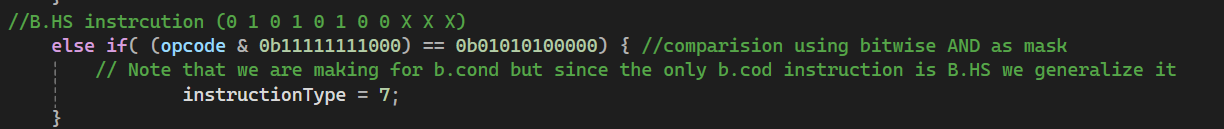
\includegraphics[width=1\textwidth]{screen_dumps/B.HSgeneralized.png}
    \caption{Generalized B.HS instruction}
    \label{fig:2}
\end{figure}

\subsection{Multiplexer Modules}
The multiplexer modules are responsible for selecting the correct input based on the control signals generated by the control unit. The multiplexer modules are initialized once and then called to select the correct input based on the control signals.\\
\subsubsection{Reg2 Multiplexer}
The Reg2 Multiplexer module preceeds the register file module and is responsible for selecting the correct second register input based on control signal Reg2Loc. Using an if else statement the module selects between the 20-16 bits of the instruction or the 4-0 bits of the instruction.\\

\subsubsection{ALU Multiplexer}
The ALU Multiplexer module preceeds the main ALU module and is responsible for selecting the correct ALU input based on control signals ALUSrc. Using an if else statement the module selects between the second register input or the sign extended immediate value.\\

\subsubsection{Data Multiplexer}
The Data Multiplexer module preceeds the data memory module and is responsible for selecting the correct data input to send back to the register file. Using an if else statement on the control signal MemtoReg, the module selects between the ALU output or the data memory output.\\

\subsubsection{PC Multiplexer}
The PC Multiplexer module preceeds the program counter module and is responsible for selecting the correct program counter input based on various control signals. This is the most complex of the multiplexers as it has to account for the different types of branch instructions. Flags present within this multiplexer are the branch, unconditional branch, InvZero and HS flags.

The main if distinguisher is the branch flag, which is set to one if the instruction is a branch instruction. In this first if statement the module checks if the instruction is a branch instruction and will either move to more if statements or set the internal PCSrc signal to zero.\\

\begin{figure}[htbp]
    \centering
    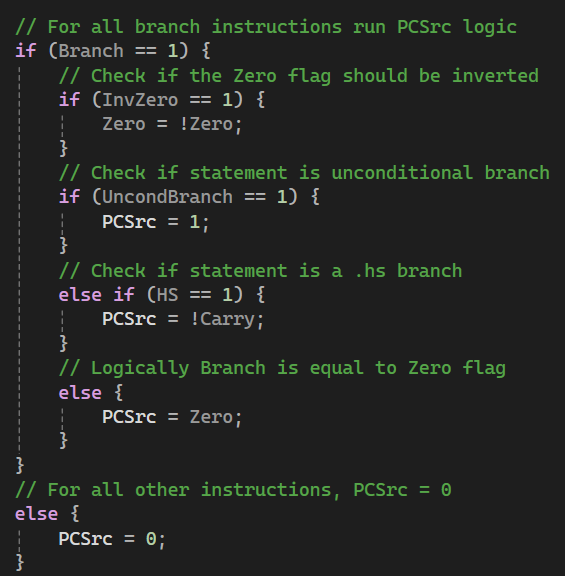
\includegraphics[width=0.6\textwidth]{screen_dumps/multiplexing_branch.png}
    \caption{Branch Multiplexing}
    \label{fig:3}
\end{figure}

\subsection{Register File Module: Registers}
The Register File module reads from and writes to the register file. It is initialized once and then called to read from or write to the register file based on the control signals generated by the control unit.\\

The RegFunction() which performs the respective read or write operation takes pointer to the register array, the read register 1 and 2, the write register and the write data and the control signal RegWrite.\\

It is important to note how register X31, also know as register XZR, is handled to be constant zero. This is done by setting hard setting the value of register XZR to zero and perfoming an extra check in the if statement when writing to registers to ensure that the register is not XZR.\\

\begin{figure}[htbp]
    \centering
    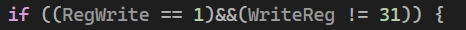
\includegraphics[width=1\textwidth]{screen_dumps/register_not_X31.png}
    \caption{Register Check !X31}
    \label{fig:4}
\end{figure}

\subsection{Sign Extend Module: SignExtend}
The Sign Extend module sign extends the immediate value of the instruction to 32 bits. The Sign Extend module is initialized once and then called to sign extend the immediate value of the instruction.\\

Here a various multiplexing takes place to set the bit field to be sign extended. The module checks the instruction type by distinguishing the bits 31, 30 and 26 of the instruction. Using these bits the instruction can be distinguished, respective bit fields can be set and the sign extension can be performed. The sign extension is simply done by taking the bit field most significant bit and copying it to the remaining bits.\\ 

\subsection{ALU Control Module: ALU\_Control}
The ALU Control module generates the ALU control signal based on the function code of the instruction. The ALU Control module is initialized once and then called to generate the ALU control signal based on the function code of the instruction.\\

It may be considered as a multiplexer as it selects the correct ALU operation based on the two ALUOp1 and ALUOp0 control signals. The module uses a if elseif statement to distinguish between the different types of instructions and the required ALU operation. Once distinguished the module sets the ALU control signal to the appropriate operation, which will then be read and used by the ALU module itself.\\

\subsection{ALU Module: ALU}
The ALU module is initialized three differnt time in the main class. The first initialization is used for the main ALU operation, the second for pc increament and the third for the branch operation.\\

The ALU module uses a simple case struct to perform the ALU operation based on the ALU control signal. Distinguisihing between the different operations and performing the respective operation. Within the ALU two flags are present, seperate from the control signals, the zero and the carry flag. These flags are initialized to zero and are only set or effected by the SUBS operation and the PASS operation.\\

The complement of the operation are fairly simple. However the SUBS operation is a bit more complex as it has to account for the carry flag and a borrow operation. So first the ALU must check wheater a borrow is needed, that is input x is smaller than input y. If a borrow is needed the ALU will will find the appropriate borrow needed based off of the y input, add the borrowed bit value to the x input and then perform the subtraction. In this case the carry flag is set to one and the zero flag is set to zero.\\

\begin{figure}[htbp]
    \centering
    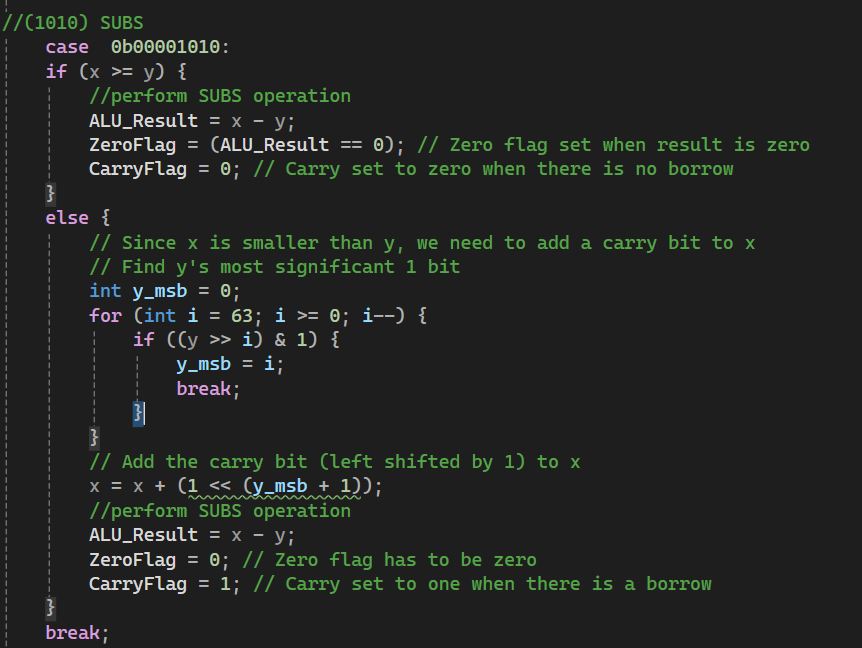
\includegraphics[width=1\textwidth]{screen_dumps/SUBS_logic.png}
    \caption{SUBS Operation Logic}
    \label{fig:5}
\end{figure}


For the PASS operation the ALU will simply pass the input y to the output, check if y is zero and pass the previous carry flag as the present carry flag.\\


\begin{figure}[htbp]
    \centering
    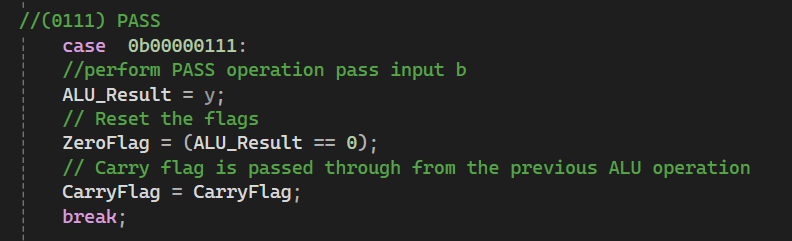
\includegraphics[width=1\textwidth]{screen_dumps/PASS_logic.png}
    \caption{PASS Operation Logic}
    \label{fig:6}
\end{figure}

\subsection{Memory Access Module: DataMemory}
The Data Memory module reads from and writes to the data memory. The Data Memory module is initialized once and then called to read from or write to the data memory based on the control signals generated by the control unit.\\

The DataMemory() initializing function is used to load the data from the .data file into the memory array. Here the file from which to read (.data) is hard coded into the function. This function takes pointer to the memory array and links the module memory to the main memory array.\\

The dmFunction() then performs the respective read or write operation. The function takes control signals MemWrite, MemRead, the WriteData ALU output and the memory address to be potentially written to or read from. If no ReadData is to be read then a zero is set to be read.\\

\section{Usage}
The simulators inputs are the .text and .data files that contain the instructions and data to be loaded into the processor. The simulator will output the results of the simulation after each cycle on the console.\\

Memory or register values can be hard coded into the simulator through the main class initialization, preceeding the simulation loop. This may be useful for testing and debugging senarios.\\

\section{Output}
The output found on the console is the mainly state of the registers and memory after each cycle. The output also includes valuable information such as the begining number of instructions, the current instruction being executed and the program counter.\\

\begin{figure}[htbp]
    \centering
    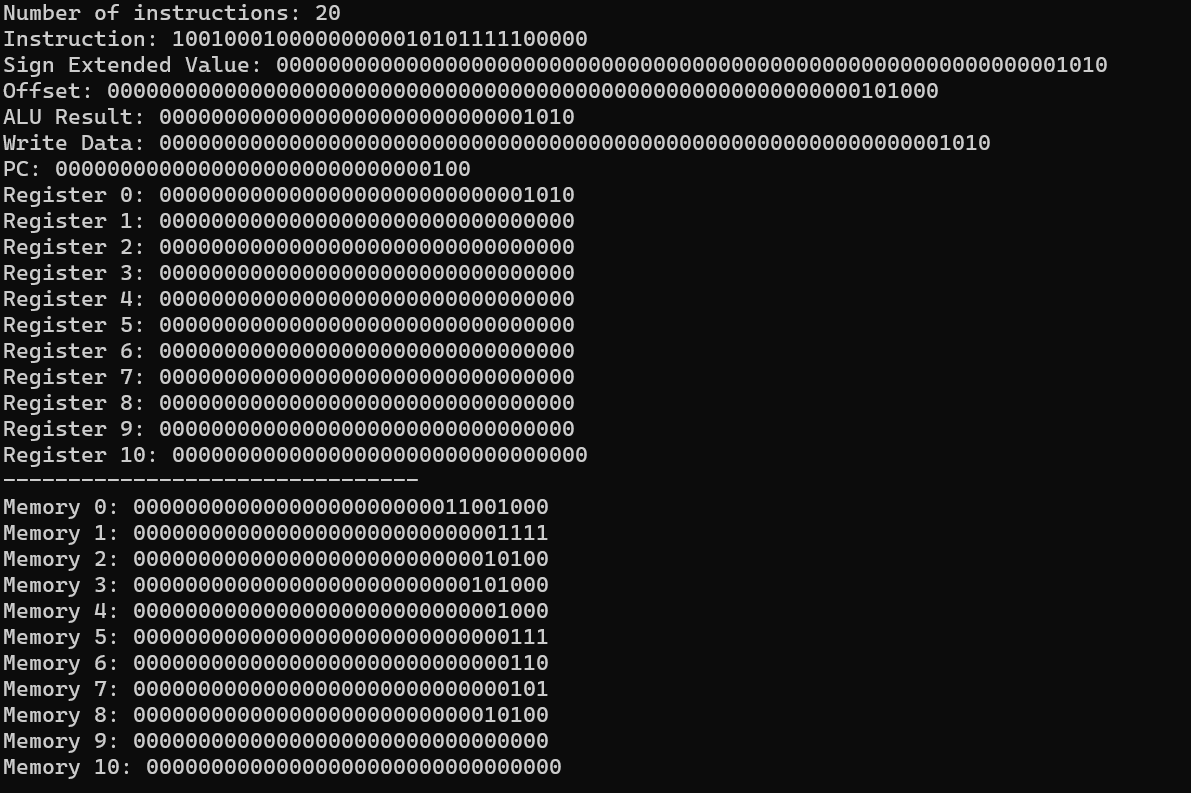
\includegraphics[width=0.8\textwidth]{screen_dumps/example_output.png}
    \caption{Output Example}
    \label{fig:7}
\end{figure}

These outputs can be used to debug the simulator and the different modules that make up the processor. The seperation between instruction is also useful to see the different stages of the instruction execution more clearly.\\

\section{Testing}
The simulator and the different instruction implementations where tested using three assembly sorce files. Which when compiled with the respective assembler gave the .text and .data input files to be loaded into the simulator.These test files all contain the assembly source, the .text and .data files and the output terminat in a .txt file. The files are as follows:\\

\subsubsection{Arithmetic}
This assembler source tests the ADD, SUB, ADDI, SUBI instructions. Here very simple arithmetic operations are performed.\\

\subsubsection{Branch}
This assembly source tests the B, B.HS, SUBS, CBZ and CBNZ instructions. ADDI is used to load the registers with values and then the branch instructions are run based on conditions off of the respective register values. Logically we each register has a differnt debugging purpose and we set 3 good regiters as flags to be checked and one bad register to be checked whose value is expected to be zero for the ideal case.\\

\subsubsection{DataTransfer}
This assembly source tests the LDURB and STURB instructions. Here we load a value into a register and then store it into memory. We then load the value from memory and store it into another register. Validating that the value was stored and loaded correctly at output.\\

\section{Bubble Sort}
The requirement of the project section 4 was to implement a bubble sort algorithm using the limited instruction set created in the single-cycle processor. The bubble sort algorithm is to sort in ascending order a list of ten 8-bit unsigned numbers stored in the data memory. Using a common test list of 200, 15, 20, 40, 8, 7, 6, 5, 20, 0. \\

The respective attempt at the bubble sort algorithm can be found in the \texttt{bubble\_sort} file where an assembly source and respectively generated .text and .data files can be found. However the bubble sort algorithm was not able to be implemented fully due to time constraints.\\

Currently the bubble sort algorithm stops running after the first iteration of each loop. That is it runs the first 20 instructions and then stops, rather than begining the inner loop. The issue is believed to be either in the PC Multiplexer module, where the branch flag is not being set correctly or else in the Bubble Sort assembly source itself. The application loads the .data correctly and the registers are being loaded correctly. It even does the first swap of the first two values correctly but doesnt seem to be able to loop back to the beginning of the inner loop.\\
  
Appart from time limitations the bubble sort algorithm attempt still brought understanding to the implementation of the branch instructions and the general logic of the processor. Showing how assembly source can be used to implement a simple algorithm and how the processor can be used to execute the algorithm.\\

Note the output of the bubble sort is aldo found in the file as a .txt file but as expected only shows the first 20 instructions and output does get sorted.\\

\section{Documentation Of Copilot Use}
Copilot was used during the development of the simulator to help with the development of the simulator. Copilot was mostly used by tabbing suggetions to generate base code for the simulator modules.\\

However, as the project progressed the use of Copilot was reduced as most LEGv8 logic was being overseen and more debugging from previous accepted prompts was having to be done rather than progression in development. Logic errors such as the bits needed to be masked in the control unit module to destiguish between the different types of instructions and the respective control signals to be set. Other areas such as the PC Multiplexer module where the PCSrc logic was not interpreted correctly and in the SignExtend module where bit field selection and multiplexing kept having consistent errors that had to be debugged.\\

The use of Copilot was rather helpful however in areas such as the ALU module where the ALU operations where correctly set and fine tunning of the SUBS and PASS operations where done. Its use also fascilitated not having to focus too much on the code and the coding language itself but rather on the logic of the processor and the different modules. A great example of this is when i had forgtten to implement the read of the .data file into the memory array and Copilot was able to suggest the correct syntax and logic to be used.\\

One further area where Copilot went on a missleading tangent was the initialzation process of the simulator. Copilot suggested that the initialization of the simulator should be done inside the main loop of the simulator. This was not an ideal case as it would eventually take up too much space and make the code less smart coded. So the initialization was moved otuside the main loop and the constructors where used to initialize the modules.\\

\section{Conclusion}
All in all this report has briefly highlighted:
\begin{itemize}
    \item The implementation of the single-cycle processor simulator and the different modules that make up the processor. 
    \item A sample showing the output of the simulator and how to interpret it.
    \item How the simulator can be used to test different assembly source files and how the respective output may be found/saved and used for debugging.
    \item Description of the test files used to test the simulator and the output of the tests.
    \item The attempt at implementing a bubble sort algorithm using the single-cycle processor and the issues faced.
    \item Documentation of the use of Copilot druing the project in aid to the development of the simulator.\\
    \pagebreak

    The implementation was fascilitated using bit uints and bit masks to distinguish between the different needed bits of the instructions.The use of the defined modules and the sequential link between them found in the main class loop implementation. Came together to form the single-cycle processor simulator. The different modules where then tested using different assembly source files and the output was interpreted to debug the simulator. Reaching the final stage of the project where a bubble sort algorithm was attempted to be implemented using the simulator. The structure of the simulator is such that it can be easily extended to support additional instructions and features. Further more may be reconstructed to support features such as pipelining and multi-cycle processors.\\
    \pagebreak
\section{Plagerism Form}
\begin{figure}[htbp]
    \centering
    
\includegraphics[width=0.8\textwidth]{screen_dumps/plagerism_form.png}
    \caption{Plagerism Form}
    \label{fig:8}
\end{figure}
\end{itemize}


\end{document}
